\iffalse
This file is protected by Copyright. Please refer to the COPYRIGHT file
distributed with this source distribution.

This file is part of OpenCPI <http://www.opencpi.org>

OpenCPI is free software: you can redistribute it and/or modify it under the
terms of the GNU Lesser General Public License as published by the Free Software
Foundation, either version 3 of the License, or (at your option) any later
version.

OpenCPI is distributed in the hope that it will be useful, but WITHOUT ANY
WARRANTY; without even the implied warranty of MERCHANTABILITY or FITNESS FOR A
PARTICULAR PURPOSE. See the GNU Lesser General Public License for more details.

You should have received a copy of the GNU Lesser General Public License along
with this program. If not, see <http://www.gnu.org/licenses/>.
\fi

%----------------------------------------------------------------------------------------
% Update the docTitle and docVersion per document
%----------------------------------------------------------------------------------------
\def\docTitle{OpenCPI\\ Rx App Guide}
\def\docVersion{1.4}
%----------------------------------------------------------------------------------------
\input{../../../../../doc/av/tex/snippets/LaTeX_Header.tex}
\date{Version \docVersion} % Force date to be blank and override date with version
\title{\docTitle}
\lhead{Rx App Guide}
%----------------------------------------------------------------------------------------
%\usepackage[T1]{fontenc} % http://tex.stackexchange.com/a/181119
\usepackage{graphicx}
\graphicspath{ {figures/} }
\usepackage{textcomp}
\lstset{ % https://tex.stackexchange.com/a/116572
  basicstyle=\ttfamily,
  columns=fullflexible,
  % frame=single,
  breaklines=true,
  showstringspaces=true,
  showspaces=true,
  postbreak=\mbox{\textcolor{red}{$\hookrightarrow$}\space},
}
\begin{document}
\maketitle
%\thispagestyle{fancy}

% AV-4723 blurb start
\begin{center}
\framebox{\parbox{0.8\linewidth}{\centering
\textcolor{red}{WARNING:}
Run-time failures have been observed for several unit tests and applications on PCIe-based platforms.
The work around requires modifying the \textbf{buffersize} attribute of the PL to PS (egress) boundary connection, as defined in the OAS. An example for modifying the OAS for executing on PCIe-based platforms is provided in a below section.

% INCLUDE IN AFFECTED UNIT TESTS DOCUMENTATION
%Specifically, the following XML change must be made to resolve this issue for the unit tests and reference applications:\\
%\begin{lstlisting}[showspaces=false]
%  <Connection>
%   <Port Instance="last_PL_worker" Name="out"/>
%   <Port Instance="first_PS_worker" Name="in" Buffersize="8192" Buffercount="4"/>
%  </Connection>
%\end{lstlisting}

% INCLUDE IN FIR_COMPLEX_SSE.TEST UNIT TEST DOCUMENTATION
%An additional change is required for fir\_complex\_sse.test, in that the fir\_complex\_sse.hdl's messageSize property must be be reduced from 8192 to 4096.\\ \medskip
%\begin{lstlisting}[showspaces=false]
%  <property name='messageSize' value='4096'>
%\end{lstlisting}

\PackageWarning{}{AV-4723} }}
\end{center}
% AV-4723 blurb end
\newpage

	\begin{center}
	\textit{\textbf{Revision History}}
		\begin{table}[H]
		\label{table:revisions} % Add "[H]" to force placement of table
			\begin{tabularx}{\textwidth}{|c|X|l|}
			\hline
			\rowcolor{blue}
			\textbf{Revision} & \textbf{Description of Change} & \textbf{Date} \\
		    \hline
		    v1.1 & Initial Release & 3/2017 \\
		    \hline
		    v1.2 & Updated for OpenCPI Release 1.2 & 8/2017 \\
			\hline
			v1.3 & Updated for OpenCPI Release 1.3 & 1/2018 \\
			\hline
			v1.3.1 & Updated for OpenCPI Release 1.3.1, including FMCOMMS2/3 support & 3/2018 \\
			\hline
			v1.4 & Updated recommendations for configuring OCPI\_LIBRARY\_PATH & 9/2018 \\

			\hline
			\end{tabularx}
		\end{table}
	\end{center}

\newpage
\tableofcontents
\pagebreak
\vspace{1pc}
\hrule
\section{Document Scope}
This document describes the OpenCPI Receive demo application or ``Rx App''. It includes a description of the RX App application and instructions on how to setup the various supported hardware platforms, build and execution of the application.

\section{Supported Hardware Setups}
This app is supported on the following hardware configurations:
\begin{itemize}
  \item Zedboard/FMCOMMS2
  \item Zedboard/FMCOMMS3
  \item x86/ML605/FMCOMMS2 in FMC LPC slot
  \item x86/ML605/FMCOMMS2 in FMC HPC slot
  \item x86/ML605/FMCOMMS3 in FMC LPC slot
  \item x86/ML605/FMCOMMS3 in FMC HPC slot
  \item Matchstiq-Z1
  \item Zedboard/Zipper/MyriadRF
  \item x86/Stratix IV GX development kit (230 Edition)/Zipper/MyriadRF in HSMC A slot
  \item x86/Stratix IV GX development kit (230 Edition)/Zipper/MyriadRF in HSMC B slot
  \item x86/ML605/Zipper/MyriadRF in FMC LPC slot
  \item x86/ML605/Zipper/MyriadRF in FMC HPC slot
\end{itemize}

\section{Description}
A block diagram of the RX app (for Stratix IV GX230 / Zipper on HSMC B specifically) can be seen in Figures \ref{fig:rx_app_left} and \ref{fig:rx_app_right}. Complex samples from the ADC are ingested into the FPGA, processed, potentially timestamped, and written to file.
\pagebreak
\begin{landscape}
	\begin{figure}[H]
	 	\centering
		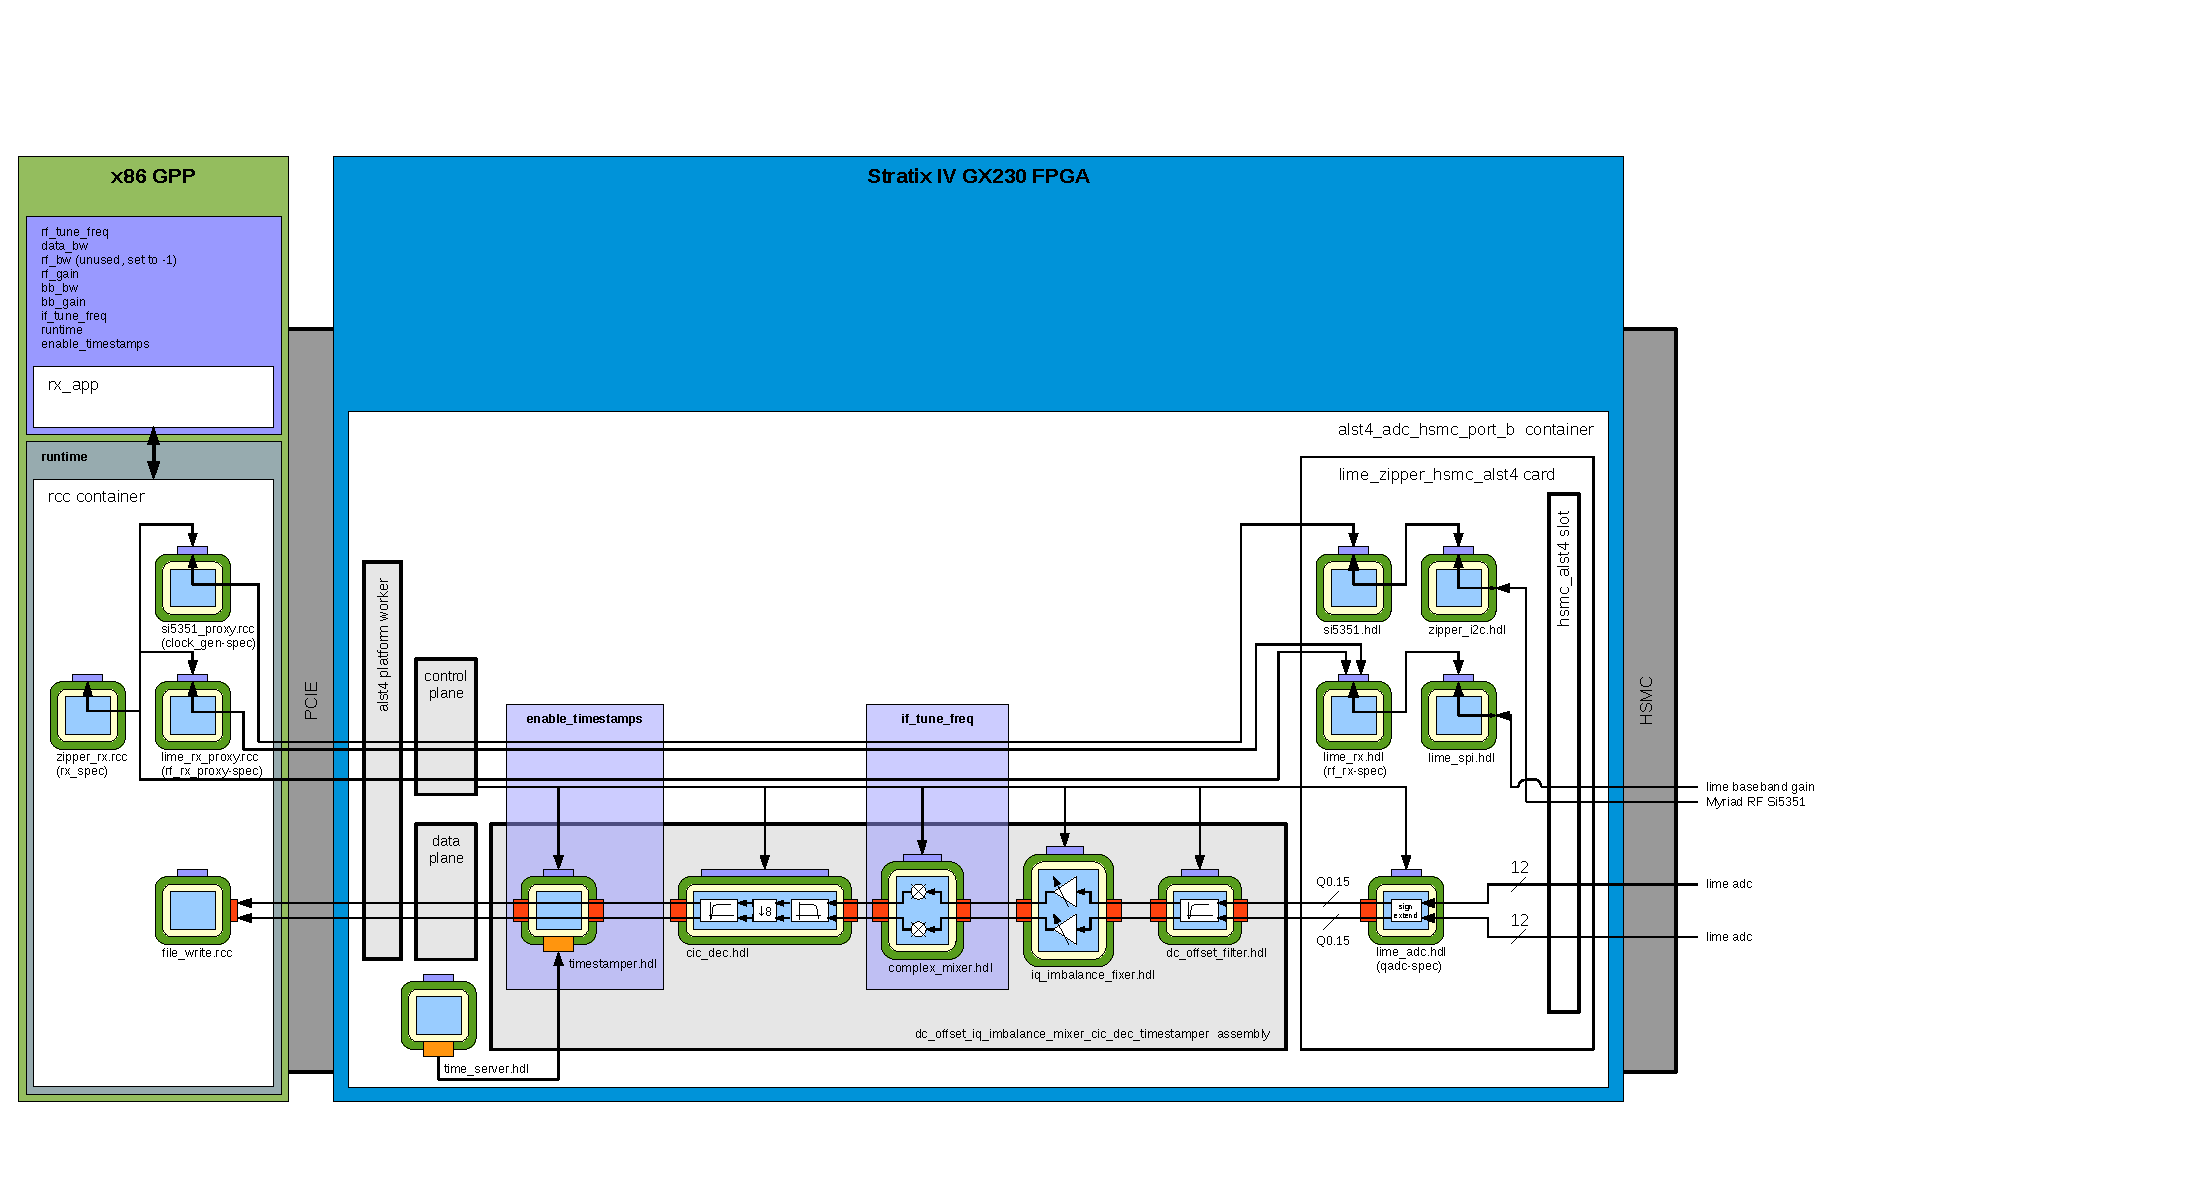
\includegraphics[scale=.65, trim={0 0 6cm 0}]{rx_app_left}
		\caption{RX App Block Diagram for Stratix IV GX230 with Zipper on HSMC B (1/2)}
		\label{fig:rx_app_left}
	\end{figure}
	\begin{figure}[H]
	 	\centering
		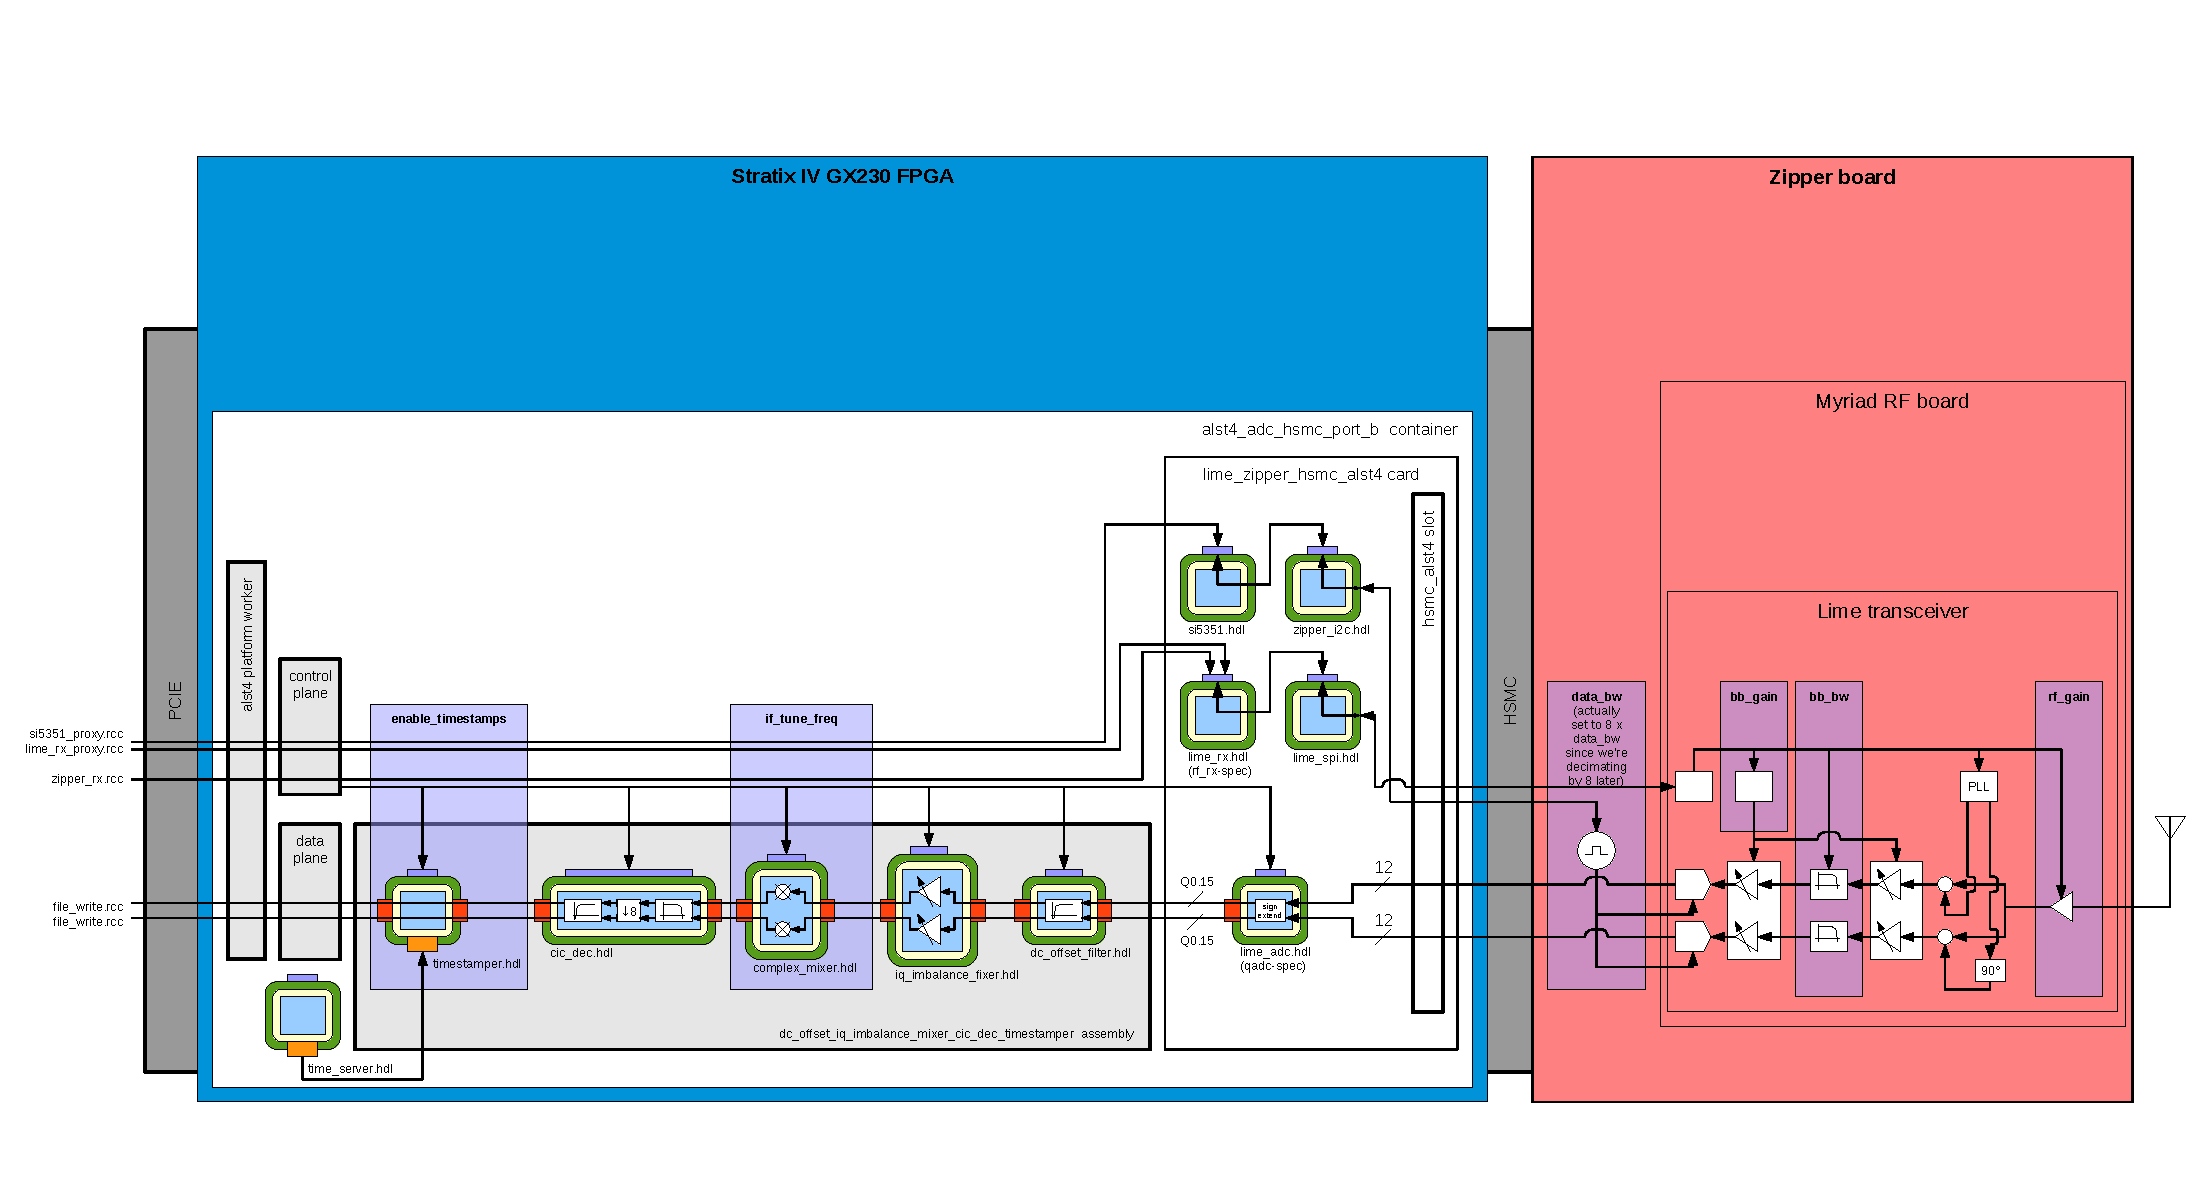
\includegraphics[scale=.65, trim={0 0 1cm 0}]{rx_app_right}
		\caption{RX App Block Diagram for Stratix IV GX230 with Zipper on HSMC B (2/2)}
		\label{fig:rx_app_right}
	\end{figure}
\end{landscape}

\section{Building the Application}
\subsection{Common Application Worker Dependencies}
The following application workers, sorted by component library name, must be built prior to building the RX application assembly. See Appendix A for the parameter configurations used in the application, and see the individual component datasheets for more information.\par\bigskip
	\begin{minipage}[t]{.5\textwidth}
	\begin{itemize}
		\item ocpi.core
			\subitem file\_write.rcc
		\item ocpi.assets.util\_comps
			\subitem timestamper.hdl
		\item ocpi.assets.dsp\_comps
			\subitem cic\_dec.hdl
			\subitem complex\_mixer.hdl
			\subitem iq\_imbalance\_fixer.hdl
			\subitem dc\_offset\_filter.hdl
	\end{itemize}
	\end{minipage}

\subsection{Hardware-Specific Worker Dependencies}
The following device and proxy workers, sorted by component library name, must be built prior to building the RX application assembly. See Appendix A for the parameter configurations used in the application, and see the individual component datasheets for more information and build instructions.\par\bigskip
	\begin{minipage}[t]{.33\textwidth}
	\textbf{Matchstiq-Z1}
	\begin{itemize}
		\item ocpi.assets.devices
			\subitem lime\_adc.hdl
			\subitem lime\_rx\_proxy.rcc
			\subitem lime\_rx.hdl
			\subitem lime\_spi.hdl
			\subitem pca9535.hdl
			\subitem si5338\_proxy.rcc
			\subitem si5338.hdl
			\subitem tmp100\_proxy.rcc
			\subitem tmp100.hdl
		\item ocpi.assets.platforms.matchstiq\_z1.devices
			\subitem matchstiq\_z1\_rx.rcc
			\subitem matchstiq\_z1\_avr\_proxy.rcc
			\subitem matchstiq\_z1\_avr.hdl
			\subitem matchstiq\_z1\_pca9535\_proxy.rcc
			\subitem matchstiq\_z1\_i2c.hdl
	\end{itemize}
	\end{minipage}
	\begin{minipage}[t]{.33\textwidth}
	\textbf{Zipper/MyriadRF Card}
	\begin{itemize}
		\item ocpi.assets.devices
			\subitem lime\_adc.hdl
			\subitem lime\_rx\_proxy.rcc
			\subitem lime\_rx.hdl
			\subitem lime\_spi.hdl
			\subitem si5351\_proxy.rcc
			\subitem si5351.hdl
	\end{itemize}
	\begin{itemize}
		\item ocpi.assets.cards
			\subitem zipper\_rx.rcc
	\end{itemize}
	\end{minipage} \medskip
	\begin{minipage}[t]{.33\textwidth}
	\textbf{FMCOMMS2/3 Cards}
	\begin{itemize}
		\item ocpi.assets.devices
			\subitem ad9361\_adc.hdl
			\subitem ad9361\_adc\_sub.hdl
			\subitem ad9361\_config.hdl
			\subitem ad9361\_config\_proxy.rcc
			\subitem ad9361\_dac.hdl
			\subitem ad9361\_dac\_sub.hdl
			\subitem ad9361\_data\_sub.hdl
			\subitem ad9361\_spi.hdl
	\end{itemize}
	\begin{itemize}
		\item ocpi.assets.cards
			\subitem fmcomms\_2\_3\_i2c.hdl
			\subitem fmcomms\_2\_3\_rx.rcc
	\end{itemize}

	\end{minipage} \medskip

\subsection{Platform-Specific Dependencies}

Platform support for the Matchstiq-Z1, Zedboard, Stratix IV, ML605 must also be built prior to building the RX application assembly. See the respective Platform Data Sheet for more information and build instructions.
\newpage

\subsection{HDL Assembly and HDL Container}
The FPGA portion of the application consists of the dc\_offset\_iq\_imbalance\_mixer\_cic\_dec\_timestamper HDL assembly and the appropriate  Matchstiq-Z1/Zedboard/Stratix IV/ML605 HDL container file. The HDL assembly instances the signal processing and timestamping components. The HDL container has three primary functions in this application:
\begin{itemize}
	\item[1)] Connects HDL assembly input to the ADC hardware for gathering IQ data
	\item[2)] Connects HDL assembly output to the processor for writing data to disk
	\item[3)] Instances command and control SPI/I2C HDL Device Workers required to configure the RF front end
\end{itemize}
\begin{landscape}
\subsection{Performance and Resource Utilization}
\input{../../../hdl/assemblies/dc_offset_iq_imbalance_mixer_cic_dec_timestamper/utilization.inc}
\end{landscape}

\subsection{Executable}
\noindent The software portion of the application consists of a C++ program written using the OpenCPI C++ API, RCC endpoint proxy workers for command and control functionality, and the file\_write.rcc RCC app worker for capturing data. For more implementation details on the endpoint proxy, see the matchstiq\_z1\_rx.rcc,  zipper\_rx.rcc, or fmcomms\_2\_3\_rx.rcc component datasheets. The C++ program instantiates and OpenCPI application object using one of the application XML files: rx\_fmcomms\_2\_app.xml, rx\_fmcomms\_3\_app.xml, rx\_matchstiq\_z1\_app.xml, rx\_zipper\_app.xml. Each of these files contain all of the property settings for the components in the application, except the configuration of the endpoint proxy for controlling RF hardware. These settings are passed on the command line to the approriate endpoint proxy worker and set using the ACI.\par\bigskip
To build for the host platform (centos6/centos7 - which is the case if ML605 or Stratix IV platform is intended to be used), run the following commands from the \textit{rx\_app} directory:\par\medskip
\texttt{ ocpidev build}\par\medskip
\noindent To build for the Zedboard or Matchstiq-Z1 (which run the xilinx13\_3 PetaLinux operating system), run the following command from the \textit{rx\_app} directory:\par\medskip
\texttt{ ocpidev build --rcc-platform xilinx13\_3 }\par\medskip
\noindent For optimal throughput, the file write RCC component writes directly to RAM via a Linux RAMdisk at runtime, and the application copies the data from RAM to a file in the application directory (odata/rx\_app\_raw.out) RX data capture is complete. The executable creates an additional shortened copy of this data (odata/rx\_app\_shortened.out) which omits some number of bytes from the beginning of the data. This is done because some of the components include feedback loops which require some setup time before functioning as desired.
\section{Testing the Application}
\subsection{Sample Test Setup}
\noindent To verify functionality of the application, a transmitter broadcasting a known signal is needed. Optionally, a spectrum analyzer to compare the transmitter output to the received data is a useful verification tool.\par\medskip
\noindent Figure \ref{fig:rx_app_test_setup} shows an example test setup for the RX app. It uses GNUradio and the Ettus N210 SDR to inject data into the Platform Under Test. GNUradio is available to download in the default CENTOS 7 repository, and a sample block diagram for transmitting random FSK data is included with this application (gnuradio/usrp\_fsk.grc). The transmitter output is also split off to a spectrum analyzer.\par\bigskip
\noindent A recommended alternative to using the Ettus N210 would be an arbitrary RF signal generator.
	\begin{figure}[H]
	 	\centering
		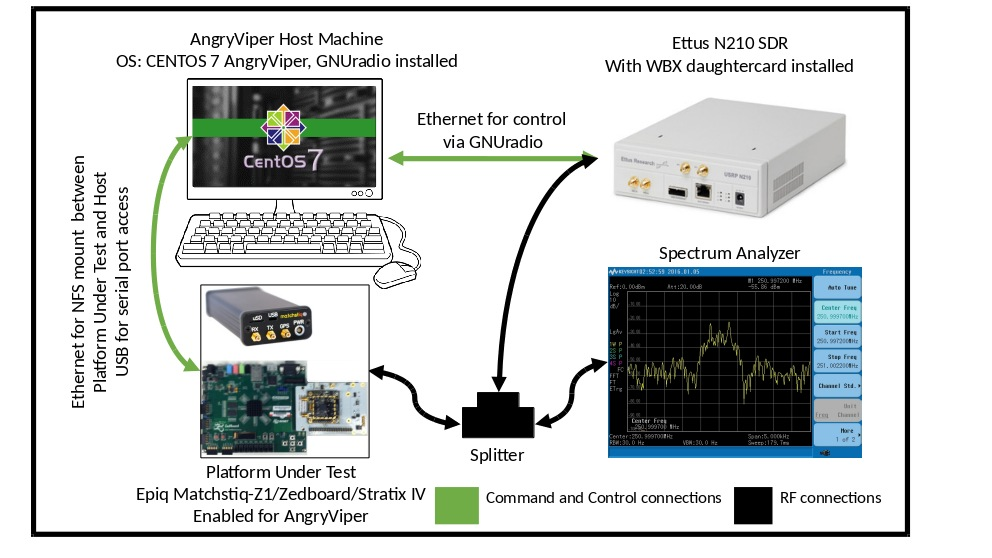
\includegraphics[scale=.55]{rx_app_test_setup}
		\caption{RX App Test Setup}
		\label{fig:rx_app_test_setup}
	\end{figure}
\subsection{make show}
\noindent In order to test the application, \texttt{make show} can be run from the \texttt{applications/rx\_app} directory. This provides instructions (for Zynq-Based Platforms) for setting \texttt{OCPI\_LIBRARY\_PATH} on the hardware platform and then running the application. Finally, it explains how to verify the output data on the development computer. The following sections provide further insight into these instructions.
\subsection{Artifacts}
\noindent Before running the application, the location of the required deployable artifacts must be specified in the OCPI\_LIBRARY\_PATH environment variable. Each RCC worker and the FPGA image exist as an artifact which should be included. Furthermore, artifacts differ depending on which mode the application is to be run in. Appendix B includes a list of the artifacts required for each platform and mode.
\newpage
\subsection{Arguments to executable}
\noindent There are eleven arguments to the RX app executable. They primarily configure the RF front end of the Platform Unit Test using the matchstiq\_z1\_rx.rcc/zipper\_rx.rcc components. Additionally, the application can be configured by setting properties in the application XML file: rx\_app.xml. Descriptions of properties can be found in the individual component datasheets. Valid ranges for each argument can be printed out by running the executable with no arguments.\par\medskip

\noindent The arguments to the executable are summarized in the below table: \\ \\
	\begin{tabular}{|l|l|}
	\hline
	\rowcolor{blue}
	Argument & Description\\
	\hline
	rf\_tune\_freq & RF (analog) tuning frequency in MHz\\
	\hline
	data\_bw & Effective sample rate of the frontend ADC (as well as the data being written to file) in MS/s\\
	\hline
	rf\_bw & Analog RF filter bandwidth in MHz\\
	\hline
	rf\_gain & RF (analog) gain in dB\\
	\hline
	bb\_bw & Analog filter bandwidth of the basebanded (downconverted) signal path in MHz\\
	\hline
	bb\_gain & Gain (analog) of basebanded (downconverted) signal path in dB\\
	\hline
	if\_tune\_freq & Tuning frequency in MHz of the HDL mixer which mixes (downconverts) the digitized data stream\\
	\hline
	runtime & Runtime of app in seconds\\
	\hline
	enable\_timestamps & Enable timestamp insertion in between messages\\
	\hline
	frontend     & Only required for Zedboard or ML605, (FMCOMMS2 or FMCOMMS3 or zipper) \\
	\hline
	sma\_channel & (optional) specify which PCB SMA is used when FMCOMMS2/3 is used (RX1A or RX2A) \\
	\hline
	\end{tabular} \medskip

\noindent\textcolor{red}{WARNING:}
Run-time failures have been observed for several unit tests and applications on PCIe-based platforms. The work around requires modifying the \textbf{buffersize} attribute of the PL to PS (egress) boundary connection, as defined in the OAS. \\
While the explicit PS to PL connection is explicitly define, the \textbf{buffersize} must be changed from 16352 to 8192, as shown in the example below:
\begin{lstlisting}[showspaces=false]
<Connection>
  <Port Instance="timestamper" Name="out" Buffercount="2"/>
  <Port Instance="file_write" Name="in" Buffersize="8192" Buffercount="7"/>
</Connection>
\end{lstlisting}

\subsection{Library Path Requirements}
\noindent Prior to running the application, the environment variable OCPI\_LIBRARY\_PATH must be configure, such that, all of the Rx application's run-time artifacts can be located. OpenCPI conveniently provides access to a project's run-time artifacts at the top-level of each project in a directory called artifacts. Reference the OpenCPI Application Development Guide for more about OCPI\_LIBRARY\_PATH. \par\medskip
\noindent Note that the ML605 and Stratix IV GX230 hardware setups require the intended slot-specific bitstream's file location to be first in OCPI\_LIBRARY\_PATH. This is necessary because ocpirun's artifact compatibility test does not currently differentiate between slot-connected device workers for multiple bitstreams that contain the same device worker, in the scenario where what differentiates the bitstreams is the device worker's slot connectivity. \par\medskip

\noindent The following are recommendations for configuring the OCPI\_LIBRARY\_PATH based on the platform, the use of a daughter card and specific slot that card is installed. For all recommendations:
\begin{itemize}
  \item All paths are relative to the applications/rx\_app/ directory.
  \item It is assumed (for PCI/host platforms) that the \code{core} and \code{assets} projects are named as such and exist in the same parent directory.\\
\end{itemize}

\noindent\textbf{Recommended Library Path for Matchstiq-Z1 or Zedboard}\\

\noindent
For these platforms, follow the instructions contained in the Rx application's Makefile. They can be viewed by opening the Makefile in an editor, or by executing ``\code{make show}'' from within the assets/applications/rx\_app/.
\\

\newpage
\noindent\textbf{Recommended Library Path for ML605/FMCOMMS2/3 in FMC HPC}\\

\noindent
\verb|OCPI_LIBRARY_PATH=../../artifacts/ocpi.assets.dc_offset_iq_imbalance_mixer_cic_dec_timestamper_\| \\
\verb|ml605_cfg_1rx_0tx_fmcomms_2_3_hpc_lvds_cnt_1rx_0tx_thruasm_fmcomms_2_3_hpc_LVDS_ml605.hdl.0.ml605.gz\| \\
\verb|:../../../core/artifacts:../../artifacts| \\
\par\medskip

\noindent\textbf{Recommended Library Path for ML605/FMCOMMS2/3 in FMC LPC}\\

\noindent
\verb|OCPI_LIBRARY_PATH=../../artifacts/ocpi.assets.dc_offset_iq_imbalance_mixer_cic_dec_timestamper_\| \\
\verb|ml605_cfg_1rx_0tx_fmcomms_2_3_lpc_lvds_cnt_1rx_0tx_thruasm_fmcomms_2_3_lpc_LVDS_ml605.hdl.0.ml605.gz \| \\
\verb|:../../../core/artifacts:../../artifacts| \\
\par\medskip

\noindent\textbf{Recommended Library Path for ML605/Zipper in FMC HPC}\\

\noindent
\verb|OCPI_LIBRARY_PATH=../../artifacts/ocpi.assets.dc_offset_iq_imbalance_mixer_cic_dec_timestamper_\| \\
\verb|ml605_ml605_zipper_fmc_hpc_rx_cnt_1rx_0tx_thruasm_zipper_hpc_ml605.hdl.0.ml605.gz\| \\
\verb|:../../../core/artifacts:../../artifacts| \\
\par\medskip

\noindent\textbf{Recommended Library Path for ML605/Zipper in FMC LPC}\\

\noindent
\verb|OCPI_LIBRARY_PATH=../../artifacts/ocpi.assets.dc_offset_iq_imbalance_mixer_cic_dec_timestamper_\| \\
\verb|ml605_ml605_zipper_fmc_lpc_rx_cnt_1rx_0tx_thruasm_zipper_lpc_ml605.hdl.0.ml605.gz\| \\
\verb|:../../../core/artifacts:../../artifacts| \\
\par\medskip

\noindent\textbf{Recommended Library Path for Stratix IV GX230/Zipper in HSMC A}\\

\noindent
\verb|OCPI_LIBRARY_PATH=../../artifacts/ocpi.assets.dc_offset_iq_imbalance_mixer_cic_dec_timestamper_\| \\
\verb|alst4_alst4_zipper_hsmc_alst4_port_a_rx_cnt_1rx_0tx_thruasm_zipper_hsmc_a_alst4.hdl.0.alst4.gz\| \\
\verb|:../../../core/artifacts:../../artifacts| \\
\par\medskip

\noindent\textbf{Recommended Library Path for Stratix IV GX230/Zipper in HSMC B}\\

\noindent
\verb|OCPI_LIBRARY_PATH=../../artifacts/ocpi.assets.dc_offset_iq_imbalance_mixer_cic_dec_timestamper_\| \\
\verb|alst4_alst4_zipper_hsmc_alst4_port_b_rx_cnt_1rx_0tx_thruasm_zipper_hsmc_b_alst4.hdl.0.alst4.gz\| \\
\verb|:../../../core/artifacts:../../artifacts| \\
\par\medskip


\pagebreak
\subsection{Expected results}
\noindent A python script is included with the application for plotting the received data in both the time and frequency domain. Using the test setup shown above and the default settings for the GNUradio block diagram, run the application with the following arguments:\par\medskip

\small
\noindent\textbf{FMCOMMS2/3}
\scriptsize
\begin{verbatim}
# Usage is:
# ./target-xilinx13_3/rx_app rf_tune_freq data_bw rf_bw rf_gain bb_bw bb_gain if_tune_freq runtime enable_timestamps
  ./target-xilinx13_3/rx_app 1000         0.256   -1    12      1     -1      0.256        1       1
\end{verbatim}
\par\medskip
\small

\noindent\textbf{Matchstiq-Z1}
\scriptsize
\begin{verbatim}
# Usage is:
# ./target-xilinx13_3/rx_app rf_tune_freq data_bw rf_bw rf_gain bb_bw bb_gain if_tune_freq runtime enable_timestamps
  ./target-xilinx13_3/rx_app 1000         0.256   400   10      0.75  51      0.256        1       1
\end{verbatim}
\par\medskip
\small

\noindent\textbf{Zipper/Myriad RF card}
\scriptsize
\noindent
\begin{verbatim}
# Usage is:
# ./target-centos7/rx_app rf_tune_freq data_bw rf_bw rf_gain bb_bw bb_gain if_tune_freq runtime enable_timestamps frontend
  ./target-centos7/rx_app 1000         0.256   -1    6       0.75  51      0.256        1       1                  zipper
\end{verbatim}
\small
\par\medskip
\noindent The output file can then be plotted with the python script with the following syntax and the output can be seen below:\par\medskip
\noindent\texttt{python ./scripts/plotAndFftAndTime.py odata/rx\_app\_raw.out complex 18000 256000 16352}\par
	\begin{figure}[h]
	 	\centering
		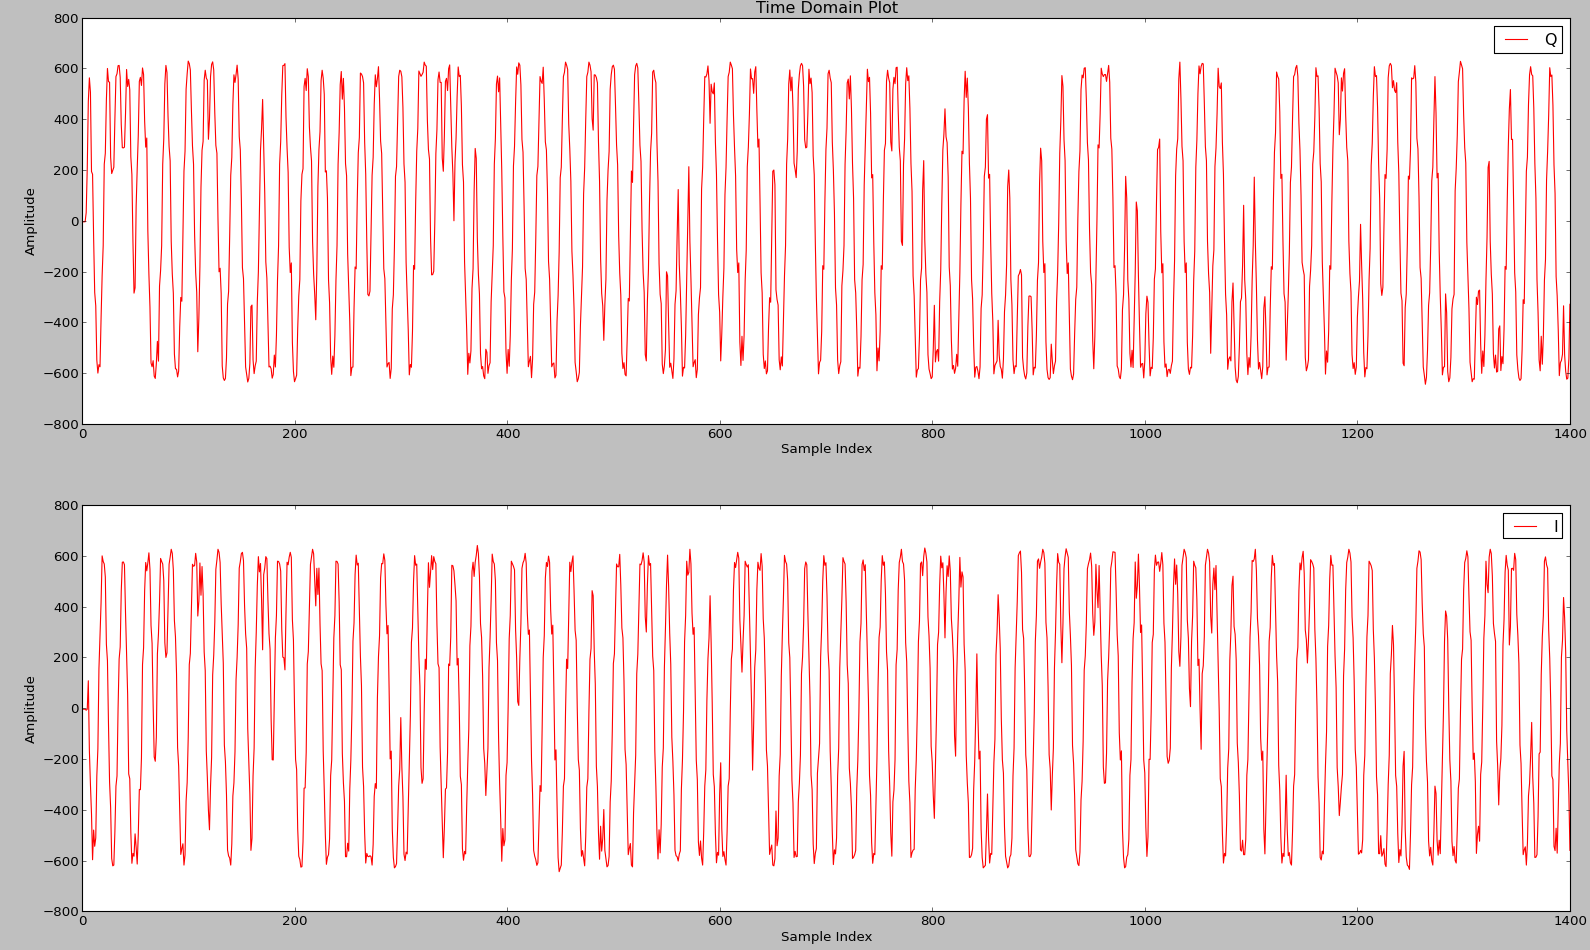
\includegraphics[scale=.2]{rx_app_iq_plot}
		\label{fig:rx_app_iq_plot}
	\end{figure}
	\begin{figure}[h]
	 	\centering
		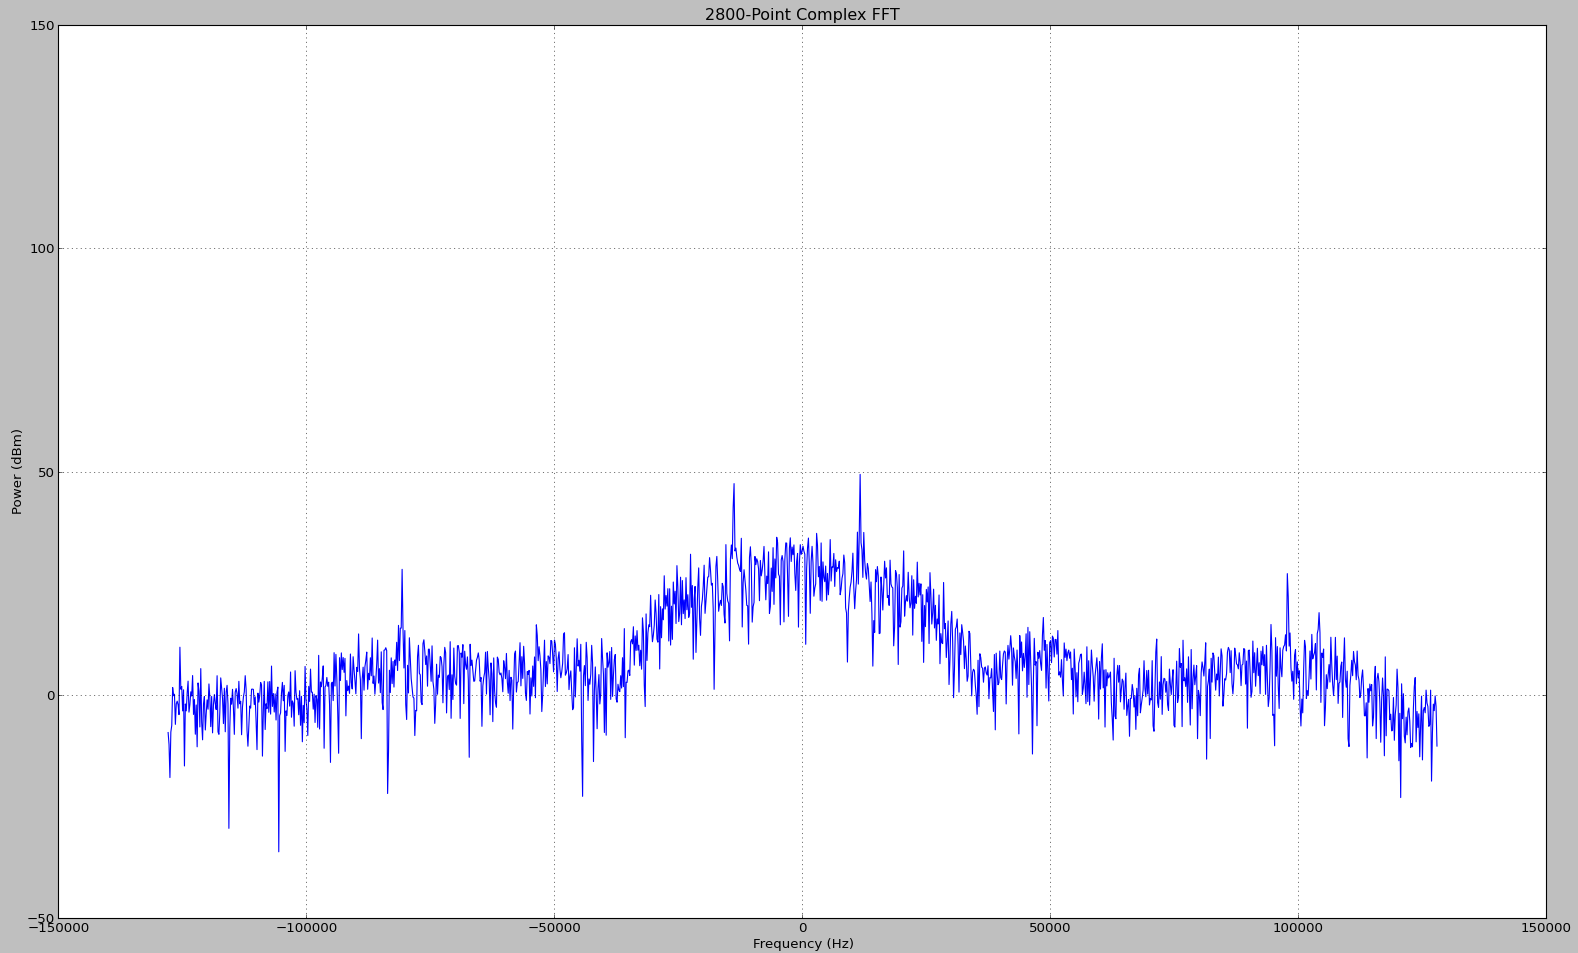
\includegraphics[scale=.2]{rx_app_fft_plot}
		\caption{Output of RX app}
		\label{fig:rx_app_fft_plot}
	\end{figure}
\noindent Alternatively, the shortened file can be plotted which will ignore optionally unwanted startup data:\par\medskip
\noindent\texttt{python ./scripts/plotAndFftAndTime.py odata/rx\_app\_shortened.out complex 18000 256000 16352}\par\medskip
\noindent The default sample rate for the GNUradio block diagram is 512 kS/s. It is recommended that when using RX app with this input signal that a sample rate close to 512 kS/s be used. Higher sample rates are still valid, but may produce plots that look drastically different than those shown here.\par\medskip
\newpage
\noindent Timestamps are embedded, optionally, in the output file, and in addition to plotting, the script parses out and prints the timestamps. An example output gathered using the syntax above:\par\medskip
\scriptsize\noindent\texttt{Timestamp at index: 000000000 :  1.0728292 Seconds: 0x1 Fraction: 0x12a4eec4  \\
Timestamp at index: 000008180 :  1.0887978 Seconds: 0x1 Fraction: 0x16bb73ba ('Delta: 0.0159686', 'Expected:, 0.0159688')\\
Timestamp at index: 000016360 :  1.1047664 Seconds: 0x1 Fraction: 0x1ad1f906 ('Delta: 0.0159686', 'Expected:, 0.0159688')}\par\medskip
\noindent\small A small discrepancy (+/- 10) between Delta and Expected is typical. The difference is an artifact of the resolution of the fractional part of the timestamp applied in the timestamper HDL component. More information can be found in the timestamper component datasheet.\par\medskip
\par\medskip

\subsection{Using a RF Signal Generator}
\noindent An arbitrary RF signal generator can be used with RX app instead of the Ettus N210. \\

\subsubsection{Example Hardware Setups}
\noindent\textbf{FMCOMMS2/3 card}
\begin{itemize}
  \item Signal generator is set to 2400.8 MHz with an amplitude of -40 dBm.
  \item Signal generator is connected to the FMCOMMS2/3 RX1A SMA.
\end{itemize}
\noindent\textbf{Matchstiq-Z1 platform}
\begin{itemize}
  \item Signal generator is set to 2400.8 MHz with an amplitude of -60 dBm.
  \item Signal generator is connected to the Matchstiq-Z1 RX SMA.
\end{itemize}
\noindent\textbf{Zipper card}
\begin{itemize}
  \item Signal generator is set to 2400.8 MHz with an amplitude of -40 dBm.
  \item Signal generator is connected to the Zipper's MyriadRF's RXTEST SMA.
\end{itemize}
\pagebreak
\subsubsection{Example 1 - Execution (remote system)}
An example run with an IF tune freq of 0.1 MHz would be as follows.
\\\noindent\textbf{FMCOMMS2 card}
\lstset{language=bash, backgroundcolor=\color{lightgray}, columns=flexible, breaklines=true, prebreak=\textbackslash, basicstyle=\ttfamily, showstringspaces=false,upquote=true, aboveskip=\baselineskip, belowskip=\baselineskip}
\begin{lstlisting}
SAMP_RATE_MHZ=2.5
RF_TUNE_FREQ_MHZ=2400
IF_TUNE_FREQ_MHZ=0.1
./<target>/rx_app $RF_TUNE_FREQ_MHZ $SAMP_RATE_MHZ -1 24 2.5 -1 $IF_TUNE_FREQ_MHZ 1 1 FMCOMMS2 RX1A
\end{lstlisting}
\noindent\textbf{FMCOMMS3 card}
\begin{lstlisting}
SAMP_RATE_MHZ=2.5
RF_TUNE_FREQ_MHZ=2400
IF_TUNE_FREQ_MHZ=0.1
./<target>/rx_app $RF_TUNE_FREQ_MHZ $SAMP_RATE_MHZ -1 24 2.5 -1 $IF_TUNE_FREQ_MHZ 1 1 FMCOMMS3 RX1A
\end{lstlisting}
\noindent\textbf{Matchstiq-Z1 platform}
\begin{lstlisting}
SAMP_RATE_MHZ=2.5
RF_TUNE_FREQ_MHZ=2400
IF_TUNE_FREQ_MHZ=0.1
./target-xilinx13_3/rx_app $RF_TUNE_FREQ_MHZ $SAMP_RATE_MHZ 400 10 1.25 51 $IF_TUNE_FREQ_MHZ 1 1 matchstiq_z1
\end{lstlisting}
\noindent\textbf{Zipper card}
\begin{lstlisting}
SAMP_RATE_MHZ=2.5
RF_TUNE_FREQ_MHZ=2400
IF_TUNE_FREQ_MHZ=0.1
./target-xilinx13_3/rx_app $RF_TUNE_FREQ_MHZ $SAMP_RATE_MHZ -1 6 1.25 51 $IF_TUNE_FREQ_MHZ 1 1 zipper
\end{lstlisting}
\subsubsection{Example 1 - Verification (development system)}
Verify that the signal generator tone exists at 700,000 Hz in the plotted baseband signal FFT (calculated as signal generator frequency - RF tune frequency - IF tune frequency = 2400.8 MHz - 2400 MHz - 0.1 MHz = 700,000Hz).
\begin{lstlisting}
SAMP_RATE_HZ=2500000
python ./scripts/plotAndFftAndTime.py odata/rx_app_shortened.out complex 65536 $SAMP_RATE_HZ 16352 &
\end{lstlisting}
        \begin{figure}[H]
        \begin{minipage}{.5\textwidth}
                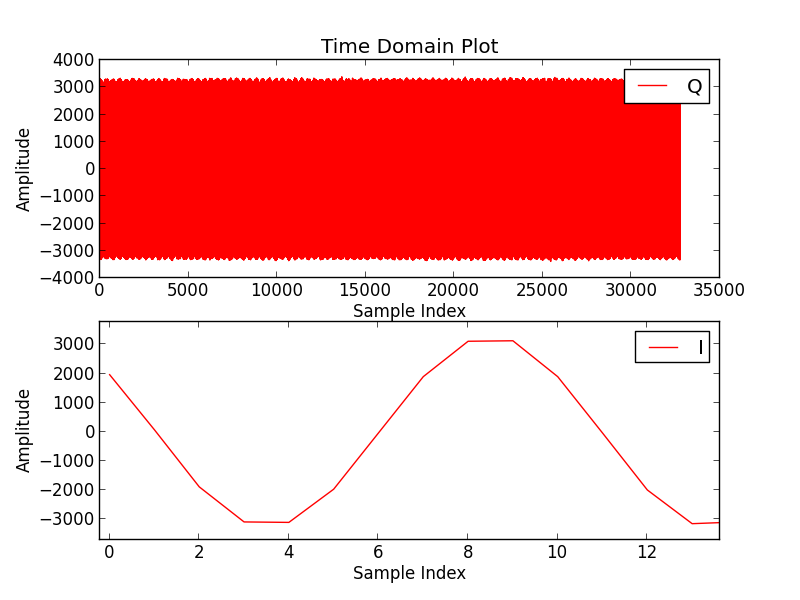
\includegraphics[width=7cm,height=5.5cm,keepaspectratio]{rx_app_sig_gen_time_domain}
                \label{fig:rx_app_sig_gen_time_domain}
        \end{minipage}%
        \begin{minipage}{.5\textwidth}
                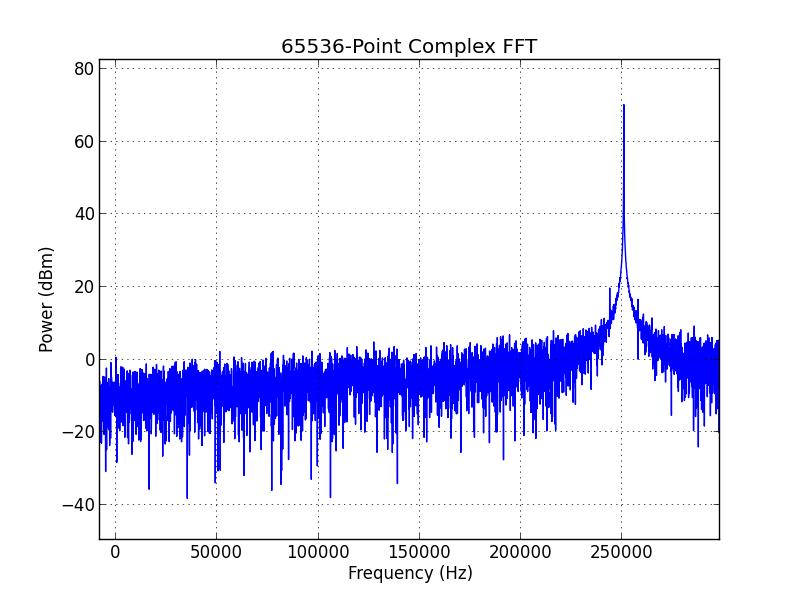
\includegraphics[width=7cm,height=5.5cm,keepaspectratio]{rx_app_sig_gen_fft}
        \end{minipage}
                \caption{Output of RX app}
                \label{fig:rx_app_sig_gen_fft}
        \end{figure}
\pagebreak
\subsubsection{Example 2 - Execution (remote system)}
An example run with an IF tune freq of 0 MHz would be as follows.
\\\noindent\textbf{FMCOMMS2 card}
\lstset{language=bash, backgroundcolor=\color{lightgray}, columns=flexible, breaklines=true, prebreak=\textbackslash, basicstyle=\ttfamily, showstringspaces=false,upquote=true, aboveskip=\baselineskip, belowskip=\baselineskip}
\begin{lstlisting}
SAMP_RATE_MHZ=2.5
RF_TUNE_FREQ_MHZ=2400
IF_TUNE_FREQ_MHZ=0
./<target>/rx_app $RF_TUNE_FREQ_MHZ $SAMP_RATE_MHZ -1 24 2.5 -1 $IF_TUNE_FREQ_MHZ 1 1 FMCOMMS2 RX1A
\end{lstlisting}
\noindent\textbf{FMCOMMS3 card}
\begin{lstlisting}
SAMP_RATE_MHZ=2.5
RF_TUNE_FREQ_MHZ=2400
IF_TUNE_FREQ_MHZ=0
./<target>/rx_app $RF_TUNE_FREQ_MHZ $SAMP_RATE_MHZ -1 24 2.5 -1 $IF_TUNE_FREQ_MHZ 1 1 FMCOMMS3 RX1A
\end{lstlisting}
\noindent\textbf{Matchstiq-Z1 platform}
\begin{lstlisting}
SAMP_RATE_MHZ=2.5
RF_TUNE_FREQ_MHZ=2400
IF_TUNE_FREQ_MHZ=0
./target-xilinx13_3/rx_app $RF_TUNE_FREQ_MHZ $SAMP_RATE_MHZ 400 10 1.25 51 $IF_TUNE_FREQ_MHZ 1 1 matchstiq_z1
\end{lstlisting}
\noindent\textbf{Zipper card}
\begin{lstlisting}
SAMP_RATE_MHZ=2.5
RF_TUNE_FREQ_MHZ=2400
IF_TUNE_FREQ_MHZ=0
./target-xilinx13_3/rx_app $RF_TUNE_FREQ_MHZ $SAMP_RATE_MHZ -1 6 1.25 51 $IF_TUNE_FREQ_MHZ 1 1 zipper
\end{lstlisting}
\subsubsection{Example 2 - Verification (development system)}
Verify that the signal generator tone exists at 800,000 Hz in the plotted baseband signal FFT (calculated as signal generator frequency - RF tune frequency - IF tune frequency = 2400.8 MHz - 2400 MHz - 0 MHz = 800,000Hz).
\begin{lstlisting}
SAMP_RATE_HZ=2500000
python ./scripts/plotAndFftAndTime.py odata/rx_app_shortened.out complex 65536 $SAMP_RATE_HZ 16352 &
\end{lstlisting}
        \begin{figure}[H]
        \begin{minipage}{.5\textwidth}
                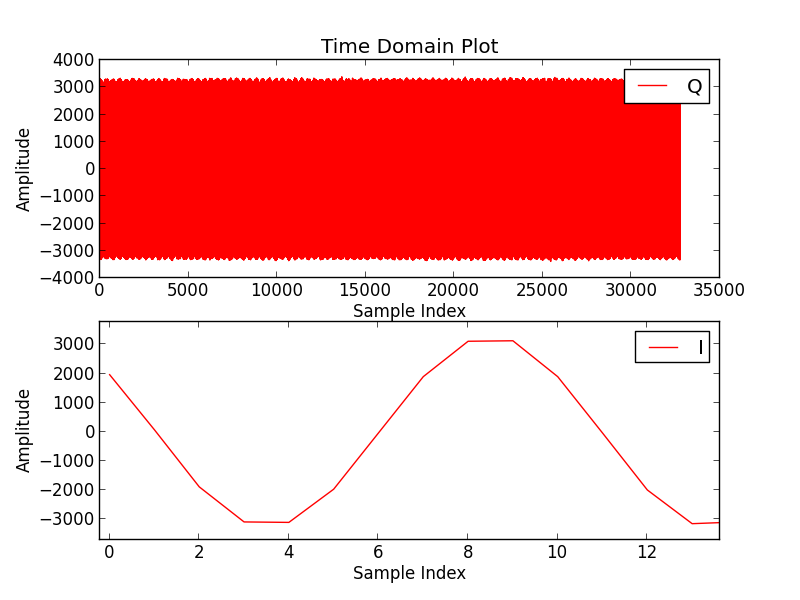
\includegraphics[width=7cm,height=5.5cm,keepaspectratio]{rx_app_sig_gen_time_domain}
                \label{fig:rx_app_sig_gen_time_domain}
        \end{minipage}%
        \begin{minipage}{.5\textwidth}
                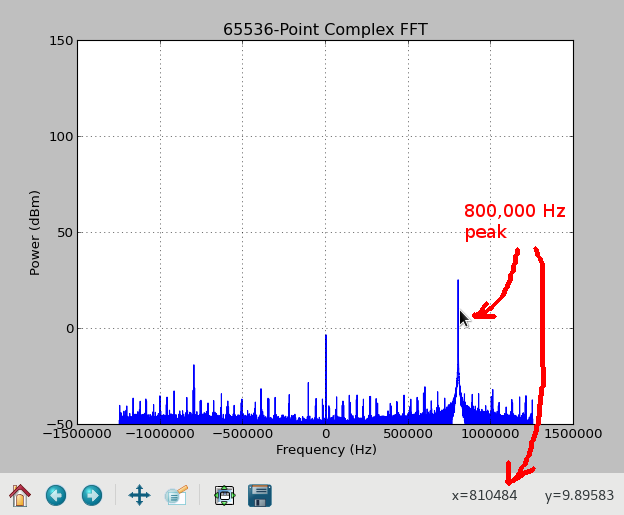
\includegraphics[width=7cm,height=5.5cm,keepaspectratio]{rx_app_sig_gen_fft_800k}
        \end{minipage}
                \caption{Output of RX app}
                \label{fig:rx_app_sig_gen_fft}
        \end{figure}
\pagebreak
\subsection{Known Issues}
\noindent
\begin{itemize}
  \item For more information on known limitations when using the Zipper-related platforms (Zedboard, Stratix IV, ML605), see the document Myriad-RF\_1\_Zipper\_Limitations included with this project.
  \item If the path \path{/var/volatile} does not exist or requires root permission to write to, you will need to modify the ACI and the application XML to use a different directory for writing data. This involves simply finding and replacing \path{/var/volatile} with a different directory in the \path{.cxx} and \path{.xml} files. Failing to make this change when necessary may result in a segmentation fault error at application runtime.
  \item  On x86 host machines with more than one Stratix IV and/or ML605s plugged into PCIe slots, this app will assume that the first found Stratix IV/ML605 has a Zipper/MyriadRF plugged in. The first found Stratix IV/ML605 will be used during execution. While there are means to address this issue, they have not been implemented for the current release.
\end{itemize}
% AV-3179
\section{Appendix A: Worker Parameters}
\begin{minipage}[t]{.5\textwidth}
	\textbf{Zedboard (with FMCOMMS2/3 card)}
	\begin{itemize}
		\item cic\_dec.hdl
			\subitem N = 3
			\subitem M = 1
			\subitem R = 8
			\subitem DIN\_WIDTH = 16
			\subitem ACC\_WIDTH = 25
			\subitem DOUT\_WIDTH = 16
		\item complex\_mixer.hdl
			\subitem NCO\_DATA\_WIDTH\_p = 12
			\subitem INPUT\_DATA\_WIDTH\_p = 12
			\subitem CORDIC\_STAGES\_p = 16
			\subitem PEAK\_MONITOR\_p = true
		\item iq\_imbalance\_fixer.hdl
			\subitem DATA\_WIDTH\_p = 16
			\subitem ACC\_PREC\_p = 34
			\subitem PEAK\_MONITOR\_p = true
		\item dc\_offset\_filter.hdl
			\subitem DATA\_WIDTH\_p = 16
			\subitem PEAK\_MONITOR\_p = true
		\item fmcomms\_2\_3\_i2c.hdl
			\subitem CP\_CLK\_FREQ\_p = 100e6
			\subitem FMC\_GA1 = 0
			\subitem FMC\_GA0 = 0
		\item ad9361\_spi.hdl
			\subitem CP\_CLK\_FREQ\_HZ\_p = 100e6
		\item ad9361\_data\_sub.hdl
			\subitem LVDS\_p = true
			\subitem DATA\_CLK\_Delay = 3
			\subitem RX\_Data\_Delay = 0
	\end{itemize}
\end{minipage}
\begin{minipage}[t]{.5\textwidth}
	\textbf{ML605 (with FMCOMMS2/3 card in FMC HPC slot)}
	\begin{itemize}
		\item cic\_dec.hdl
			\subitem N = 3
			\subitem M = 1
			\subitem R = 8
			\subitem DIN\_WIDTH = 16
			\subitem ACC\_WIDTH = 25
			\subitem DOUT\_WIDTH = 16
		\item complex\_mixer.hdl
			\subitem NCO\_DATA\_WIDTH\_p = 12
			\subitem INPUT\_DATA\_WIDTH\_p = 12
			\subitem CORDIC\_STAGES\_p = 16
			\subitem PEAK\_MONITOR\_p = true
		\item iq\_imbalance\_fixer.hdl
			\subitem DATA\_WIDTH\_p = 16
			\subitem ACC\_PREC\_p = 34
			\subitem PEAK\_MONITOR\_p = true
		\item dc\_offset\_filter.hdl
			\subitem DATA\_WIDTH\_p = 16
			\subitem PEAK\_MONITOR\_p = true
		\item fmcomms\_2\_3\_i2c.hdl
			\subitem CP\_CLK\_FREQ\_p = 125e6
			\subitem FMC\_GA1 = 0
			\subitem FMC\_GA0 = 0
		\item ad9361\_spi.hdl
			\subitem CP\_CLK\_FREQ\_HZ\_p = 125e6
		\item ad9361\_data\_sub.hdl
			\subitem LVDS\_p = true
			\subitem DATA\_CLK\_Delay = 2
			\subitem RX\_Data\_Delay = 0
	\end{itemize}
\end{minipage}

\begin{minipage}[t]{.5\textwidth}
	\textbf{ML605 (with FMCOMMS2/3 card in FMC LPC slot)}
	\begin{itemize}
		\item cic\_dec.hdl
			\subitem N = 3
			\subitem M = 1
			\subitem R = 8
			\subitem DIN\_WIDTH = 16
			\subitem ACC\_WIDTH = 25
			\subitem DOUT\_WIDTH = 16
		\item complex\_mixer.hdl
			\subitem NCO\_DATA\_WIDTH\_p = 12
			\subitem INPUT\_DATA\_WIDTH\_p = 12
			\subitem CORDIC\_STAGES\_p = 16
			\subitem PEAK\_MONITOR\_p = true
		\item iq\_imbalance\_fixer.hdl
			\subitem DATA\_WIDTH\_p = 16
			\subitem ACC\_PREC\_p = 34
			\subitem PEAK\_MONITOR\_p = true
		\item dc\_offset\_filter.hdl
			\subitem DATA\_WIDTH\_p = 16
			\subitem PEAK\_MONITOR\_p = true
		\item fmcomms\_2\_3\_i2c.hdl
			\subitem CP\_CLK\_FREQ\_p = 125e6
			\subitem FMC\_GA1 = 1
			\subitem FMC\_GA0 = 0
		\item ad9361\_spi.hdl
			\subitem CP\_CLK\_FREQ\_HZ\_p = 125e6
		\item ad9361\_data\_sub.hdl
			\subitem LVDS\_p = true
			\subitem DATA\_CLK\_Delay = 2
			\subitem RX\_Data\_Delay = 0
	\end{itemize}
\end{minipage}
\begin{minipage}[t]{.5\textwidth}
	\textbf{Matchstiq-Z1}
	\begin{itemize}
		\item cic\_dec.hdl
			\subitem N = 3
			\subitem M = 1
			\subitem R = 8
			\subitem DIN\_WIDTH = 16
			\subitem ACC\_WIDTH = 25
			\subitem DOUT\_WIDTH = 16
		\item complex\_mixer.hdl
			\subitem NCO\_DATA\_WIDTH\_p = 12
			\subitem INPUT\_DATA\_WIDTH\_p = 12
			\subitem CORDIC\_STAGES\_p = 16
			\subitem PEAK\_MONITOR\_p = true
		\item iq\_imbalance\_fixer.hdl
			\subitem DATA\_WIDTH\_p = 16
			\subitem ACC\_PREC\_p = 34
			\subitem PEAK\_MONITOR\_p = true
		\item dc\_offset\_filter.hdl
			\subitem DATA\_WIDTH\_p = 16
			\subitem PEAK\_MONITOR\_p = true
		\item lime\_adc.hdl
			\subitem DRIVE\_CLK\_p = false
			\subitem USE\_CLK\_IN\_p = false
			\subitem USE\_CTL\_CLK\_p = false
			\subitem USE\_CLK\_OUT\_p = true
		\item si5338.hdl
			\subitem CLKIN\_PRESENT\_p = true
			\subitem CLKIN\_FREQ\_p = 3.072e7
			\subitem XTAL\_PRESENT\_p = false
			\subitem XTAL\_FREQ\_p = 0
			\subitem OUTPUTS\_PRESENT\_p = 1,0,0,0
			\subitem INTR\_CONNECTED\_p = false
		\item matchstiq\_z1\_i2c.hdl
			\subitem NUSERS\_p = 5
			\subitem SLAVE\_ADDRESS\_p = 0x45,0x71,0x48,0x21,0x20
			\subitem CLK\_CNT\_p = 199
	\end{itemize}
\end{minipage}

\begin{minipage}[t]{.5\textwidth}
	\textbf{Zedboard (with Zipper/Myriad-RF card)}
	\begin{itemize}
		\item cic\_dec.hdl
			\subitem N = 3
			\subitem M = 1
			\subitem R = 8
			\subitem DIN\_WIDTH = 16
			\subitem ACC\_WIDTH = 25
			\subitem DOUT\_WIDTH = 16
		\item complex\_mixer.hdl
			\subitem NCO\_DATA\_WIDTH\_p = 12
			\subitem INPUT\_DATA\_WIDTH\_p = 12
			\subitem CORDIC\_STAGES\_p = 16
			\subitem PEAK\_MONITOR\_p = true
		\item iq\_imbalance\_fixer.hdl
			\subitem DATA\_WIDTH\_p = 16
			\subitem ACC\_PREC\_p = 34
			\subitem PEAK\_MONITOR\_p = true
		\item dc\_offset\_filter.hdl
			\subitem DATA\_WIDTH\_p = 16
			\subitem PEAK\_MONITOR\_p = true
		\item lime\_adc.hdl
			\subitem DRIVE\_CLK\_p = false
			\subitem USE\_CLK\_IN\_p = true
			\subitem USE\_CTL\_CLK\_p = false
			\subitem USE\_CLK\_OUT\_p = false
		\item si5351.hdl
			\subitem CLKIN\_PRESENT = true
			\subitem CLKIN\_FREQ = 3.072e7
			\subitem XTAL\_PRESENT = false
			\subitem XTAL\_FREQ = 0
			\subitem VC\_PRESENT = false
			\subitem OUTPUTS\_PRESENT = 0,0,1,1,1,1,0,0
			\subitem OEB\_MODE = low
			\subitem INTR\_CONNECTED = false
		\item zipper\_i2c.hdl
			\subitem NUSERS\_p = 2
	\end{itemize}
\end{minipage}
\begin{minipage}[t]{.5\textwidth}
	\textbf{Stratix IV GX230 (with Zipper/Myriad-RF card)}
	\begin{itemize}
		\item cic\_dec.hdl
			\subitem N = 3
			\subitem M = 1
			\subitem R = 8
			\subitem DIN\_WIDTH = 16
			\subitem ACC\_WIDTH = 25
			\subitem DOUT\_WIDTH = 16
		\item complex\_mixer.hdl
			\subitem NCO\_DATA\_WIDTH\_p = 12
			\subitem INPUT\_DATA\_WIDTH\_p = 12
			\subitem CORDIC\_STAGES\_p = 16
			\subitem PEAK\_MONITOR\_p = true
		\item iq\_imbalance\_fixer.hdl
			\subitem DATA\_WIDTH\_p = 16
			\subitem ACC\_PREC\_p = 34
			\subitem PEAK\_MONITOR\_p = true
		\item dc\_offset\_filter.hdl
			\subitem DATA\_WIDTH\_p = 16
			\subitem PEAK\_MONITOR\_p = true
		\item lime\_adc.hdl
			\subitem DRIVE\_CLK\_p = false
			\subitem USE\_CLK\_IN\_p = true
			\subitem USE\_CTL\_CLK\_p = false
			\subitem USE\_CLK\_OUT\_p = false
		\item si5351.hdl
			\subitem CLKIN\_PRESENT = true
			\subitem CLKIN\_FREQ = 3.072e7
			\subitem XTAL\_PRESENT = false
			\subitem XTAL\_FREQ = 0
			\subitem VC\_PRESENT = false
			\subitem OUTPUTS\_PRESENT = 0,0,1,1,1,1,0,0
			\subitem OEB\_MODE = low
			\subitem INTR\_CONNECTED = false
		\item zipper\_i2c.hdl
			\subitem NUSERS\_p = 2
	\end{itemize}
\end{minipage}

\begin{minipage}[t]{.5\textwidth}
	\textbf{ML605 (with Zipper/Myriad-RF card)}
	\begin{itemize}
		\item cic\_dec.hdl
			\subitem N = 3
			\subitem M = 1
			\subitem R = 8
			\subitem DIN\_WIDTH = 16
			\subitem ACC\_WIDTH = 25
			\subitem DOUT\_WIDTH = 16
		\item complex\_mixer.hdl
			\subitem NCO\_DATA\_WIDTH\_p = 12
			\subitem INPUT\_DATA\_WIDTH\_p = 12
			\subitem CORDIC\_STAGES\_p = 16
			\subitem PEAK\_MONITOR\_p = true
		\item iq\_imbalance\_fixer.hdl
			\subitem DATA\_WIDTH\_p = 16
			\subitem ACC\_PREC\_p = 34
			\subitem PEAK\_MONITOR\_p = true
		\item dc\_offset\_filter.hdl
			\subitem DATA\_WIDTH\_p = 16
			\subitem PEAK\_MONITOR\_p = true
		\item lime\_adc.hdl
			\subitem DRIVE\_CLK\_p = false
			\subitem USE\_CLK\_IN\_p = true
			\subitem USE\_CTL\_CLK\_p = false
			\subitem USE\_CLK\_OUT\_p = false
		\item si5351.hdl
			\subitem CLKIN\_PRESENT = true
			\subitem CLKIN\_FREQ = 3.072e7
			\subitem XTAL\_PRESENT = false
			\subitem XTAL\_FREQ = 0
			\subitem VC\_PRESENT = false
			\subitem OUTPUTS\_PRESENT = 0,0,1,1,1,1,0,0
			\subitem OEB\_MODE = low
			\subitem INTR\_CONNECTED = false
		\item zipper\_i2c.hdl
			\subitem NUSERS\_p = 2
	\end{itemize}
\end{minipage}\newpage

\section{Appendix B: Artifacts}
\subsection{Zedboard/FMCOMMS2/3}
	\begin{itemize}
	\item dc\_offset\_iq\_imbalance\_mixer\_cic\_dec\_timestamper\_zed\_cfg\_1rx\_0tx \\
\_fmcomms\_2\_3\_lpc\_lvds\_cnt\_1rx\_0tx\_thruasm\_fmcomms\_2\_3\_lpc\_LVDS\_zed.bitz
	\end{itemize}
	\begin{itemize}
	\begin{minipage}[t]{.5\textwidth}
	\item target-xilinx13\_3/file\_write\_s.so
	\item target-xilinx13\_3/fmcomms\_2\_3\_rx\_s.so
	\item target-xilinx13\_3/ad9361\_config\_proxy\_s.so
	\end{minipage}
	\end{itemize}
\subsection{ML605 FMCOMMS2/3 in FMC HPC}
	\begin{itemize}
	\item dc\_offset\_iq\_imbalance\_mixer\_cic\_dec\_timestamper\_ml605\_cfg\_1rx\_0tx \\
\_fmcomms\_2\_3\_hpc\_lvds\_cnt\_1rx\_0tx\_thruasm\_fmcomms\_2\_3\_hpc\_LVDS\_ml605.bitz
	\end{itemize}
	\begin{itemize}
	\begin{minipage}[t]{.5\textwidth}
	\item target-centos7/file\_write\_s.so
	\item target-centos7/fmcomms\_2\_3\_rx\_s.so
	\item target-centos7/ad9361\_config\_proxy\_s.so
	\end{minipage}
	\end{itemize}
\subsection{ML605 FMCOMMS2/3 in FMC LPC}
	\begin{itemize}
	\item dc\_offset\_iq\_imbalance\_mixer\_cic\_dec\_timestamper\_ml605\_cfg\_1rx\_0tx \\
\_fmcomms\_2\_3\_lpc\_lvds\_cnt\_1rx\_0tx\_thruasm\_fmcomms\_2\_3\_lpc\_LVDS\_ml605.bitz
	\end{itemize}
	\begin{itemize}
	\begin{minipage}[t]{.5\textwidth}
	\item target-centos7/file\_write\_s.so
	\item target-centos7/fmcomms\_2\_3\_rx\_s.so
	\item target-centos7/ad9361\_config\_proxy\_s.so
	\end{minipage}
	\end{itemize}
\subsection{Matchstiq-Z1}
	\begin{itemize}
	\item
dc\_offset\_iq\_imbalance\_mixer\_cic\_dec\_timestamper\_matchstiq\_z1\_matchstiq\_z1\_rx\_cnt\_1rx\_0tx\_thruasm\_matchstiq\_z1.bitz
	\end{itemize}
	\begin{itemize}
	\begin{minipage}[t]{.5\textwidth}
	\item target-xilinx13\_3/file\_write\_s.so
	\item target-xilinx13\_3/matchstiq\_z1\_rx\_s.so
	\item target-xilinx13\_3/lime\_rx\_proxy\_s.so
	\end{minipage}
	\begin{minipage}[t]{.5\textwidth}
	\item target-xilinx13\_3/si5338\_proxy\_s.so
	\item target-xilinx13\_3/matchstiq\_z1\_avr\_proxy\_s.so
	\item target-xilinx13\_3/tmp100\_proxy\_s.so
	\item target-xilinx13\_3/matchstiq\_z1\_pca9535\_proxy\_s.so
	\end{minipage}
	\end{itemize}
\subsection{Zedboard/Zipper}
	\begin{itemize}
	\item
dc\_offset\_iq\_imbalance\_mixer\_cic\_dec\_timestamper\_zed\_base\_cnt\_1rx\_0tx\_thruasm\_zipper\_lpc\_zed.bitz
	\end{itemize}
	\begin{itemize}
	\begin{minipage}[t]{.5\textwidth}
	\item target-xilinx13\_3/file\_write\_s.so
	\item target-xilinx13\_3/zipper\_rx\_s.so
	\end{minipage}
	\begin{minipage}[t]{.5\textwidth}
	\item target-xilinx13\_3/lime\_rx\_proxy\_s.so
	\item target-xilinx13\_3/si5351\_proxy\_s.so
	\end{minipage}
	\end{itemize}
\subsection{Stratix IV/Zipper}
	For Zipper plugged into HSMC Port A:
	\begin{itemize}
	\item
dc\_offset\_iq\_imbalance\_mixer\_cic\_dec\_timestamper\_alst4\_alst4\_zipper\_hsmc\_alst4\_port\_a \\ \_rx\_cnt\_1rx\_0tx\_thruasm\_zipper\_hsmc\_a\_alst4.bitz
 	\end{itemize}
	\noindent For Zipper plugged into HSMC Port B:
	\begin{itemize}
	\item	dc\_offset\_iq\_imbalance\_mixer\_cic\_dec\_timestamper\_alst4\_alst4\_zipper\_hsmc\_alst4\_port\_b \\ \_rx\_cnt\_1rx\_0tx\_thruasm\_zipper\_hsmc\_b\_alst4.bitz
	\end{itemize}
	\begin{itemize}
	\begin{minipage}[t]{.5\textwidth}
	\item target-centos7/file\_write\_s.so
	\item target-centos7/zipper\_rx\_s.so
	\end{minipage}
	\begin{minipage}[t]{.5\textwidth}
	\item target-centos7/lime\_rx\_proxy\_s.so
	\item target-centos7/si5351\_proxy\_s.so
	\end{minipage}
	\end{itemize}
\subsection{ML605/Zipper}
	For Zipper plugged into FMC HPC:
	\begin{itemize}
	\item
dc\_offset\_iq\_imbalance\_mixer\_cic\_dec\_timestamper\_ml605\_ml605\_zipper\_fmc\_lpc\_ \\ rx\_cnt\_1rx\_0tx\_thruasm\_zipper\_lpc\_ml605.bitz
 	\end{itemize}
	\noindent For Zipper plugged into FMC LPC:
	\begin{itemize}
	\item
dc\_offset\_iq\_imbalance\_mixer\_cic\_dec\_timestamper\_ml605\_ml605\_zipper\_fmc\_hpc\_ \\
rx\_cnt\_1rx\_0tx\_thruasm\_zipper\_hpc\_ml605.bitz
	\end{itemize}
	\begin{itemize}
	\begin{minipage}[t]{.5\textwidth}
	\item target-centos7/file\_write\_s.so
	\item target-centos7/zipper\_rx\_s.so
	\end{minipage}
	\begin{minipage}[t]{.5\textwidth}
	\item target-centos7/lime\_rx\_proxy\_s.so
	\item target-centos7/si5351\_proxy\_s.so
	\end{minipage}
	\end{itemize}
\end{document}
